%!TEX root = ../matcomp.tex
%!TEX encoding = UTF-8 Unicode

\subsection{Corpi convessi e norme}

Dopo aver definito il JSR, è ovviamente di notevole importanza trovare un modo per calcolarlo. 
A tale scopo introduciamo una interessante corrispondenza tra norme e ``palle'' in $\R^{n}$.

\begin{definizione}
	Un insieme $C\subset\R^{n}$ si dice \emph{corpo convesso centrato} (CCB) se è compatto, ha interno non vuoto ed è simmetrico rispetto allo $0\in\R^{n}$.
\end{definizione}

Grazie al funzionale di Minkowski (talvolta chiamato anche \emph{gauge})
$$\|x\|_{C} = \inf\{\mu>0:\; x\in \mu C\}$$
si può stabilire una dualità $C\sim \|\cdot\|_{C}$ tra norme in $\R^{n}$ e CCB. Vediamone alcune proprietà.

\begin{proposizione}
	Dati $C_{1}, C_{2}$ CCB, allora:
	\begin{itemize}
		\item $C_{1}\subseteq C_{2} \iff \|\cdot\|_{C_{1}}\geq\|\cdot\|_{C_{2}}$;
		\item $C_{1}\cap C_{2}$ è un CCB, e $\|\cdot\|_{C_{1}\cap C_{2}} = \sup\{\|\cdot\|_{C_{1}},\|\cdot\|_{C_{2}}\}$;
		\item se $t>0$, allora $tC\sim t^{-1}\|\cdot\|_{C}$; più in generale, se $A\in GL_{n}\R$ allora $A[C]\sim \|A^{-1}\cdot\|_{C}$.
	\end{itemize}
\end{proposizione}
\begin{proof}
	Il primo punto è ovvio. Per il secondo, si ha che preso $v\in\R^{n}$ vale
	\begin{align*}
		\|v\|_{C_{1}\cap C_{2}} &= \min\{r\geq0:\, v\in r(C_{1}\cap C_{2})\}
		= \min\{r\geq0:\, v \in rC_{1}, v\in rC_{2}\} \\&
		= \max\{\min\{r:\, v\in rC_{1}\}, \min\{r:\, v\in rC_{2}\}\} 
		= \max\{\|v\|_{C_{1}}, \|v\|_{C_{2}}\}.
	\end{align*}
	Per l'ultimo punto, si vede che 
		$$\|v\|_{A[C]} = \min\{r\geq0:\, v\in rA[C]\} = \min\{r\geq0:\, A^{-1}v\in rC\} = \|A^{-1}v\|_{C}.$$
\end{proof}

\begin{osservazione}
	Dato un qualsiasi insieme $A\subseteq\R^{n}$ purché limitato e con interno non vuoto, esiste il minimo CCB che lo contiene, definito da $\bigcap\{C:\, C\text{ è un CCB},\,A\subseteq C\}$.
	La condizione sull'interno non vuoto serve perché ad esempio si potrebbe pensare di fare l'intersezione infinita di rettangoli che si stringono su una retta, ottenendo un segmento che ovviamente non è un CCB.
\end{osservazione}

Grazie all'osservazione, possiamo definire un $\sup$ sui corpi convessi come segue:
$$C_{1}\vee C_{2}:=\bigcap \{C:\, C\text{ è un CCB},\, C_{1}\cup C_{2}\subseteq C\}.$$
Una definizione alternativa dal basso è quella che consiste nel prendere $C_{1}\cup C_{2}$ e farne la chiusura convessa. L'equivalenza con la definizione appena data è lasciata per esercizio. 
A livello di norme questa operazione di estremo superiore, se poniamo $C_{3} = C_{1}\vee C_{2}$, corrisponde alla norma definita da 
$$\|v\|_{C_{3}} = \max\{\|v\|:\,\|v\|\text{ è una norma $\leq$ di } \|v\|_{C_{1}}, \|v\|_{C_{2}}\},$$
ossia all'estremo inferiore (fatto considerando l'ordinamento tra norme).

Ovviamente partendo da una norma indotta da un CCB si può definire come al solito la corrispondente norma di operatore, ricordando che $C$ stesso è la palla unitaria per $\|\cdot\|_{C}$:
$$\|R\|_{C} = \|R[C]\|_{C} = \min\{r:\,R[C]\subseteq rC\}.$$

\begin{esercizio}[carino]
	Si consideri la somma di Minkowski tra CCB definita da 
	$$C_{1} + C_{2} := \{c_{1} + c_{2}:\, c_{1}\in C_{1},\, c_{2}\in C_{2}\}.$$
	A cosa corrisponde per le norme?
\end{esercizio}

Vediamo ora a cosa ci è servito introdurre la nozione di CCB e la dualità con le norme.

\begin{lemma}[chiave]
	Sia $w\in N^{*}$, e $[\rho(R_{w})]^{1/|w|} = \alpha >0$. Sia inoltre $C$ un CCB tale che $\alpha^{-1}R_{0}C, \dots, \alpha^{-1}R_{N-1}C$ sono contenuti in $C$. Allora $\tilde\rho(\mathcal R) = \alpha$, la norma $\|\cdot\|_{C}$ è estrema per $\mathcal R$ e $R_{w}$ è un \emph{prodotto ottimo} (cioè $\forall u\in N^{*},\,[\rho(R_{u})]^{1/|u|}\leq\alpha$). Inoltre necessariamente per almeno un indice $i\in N$ si ha $\alpha^{-1}R_{i}C \subsetneq \overset{\circ}{C}$.
\end{lemma}
\begin{proof}
	Vale senz'altro $\alpha\leq\tilde\rho$ per la caratterizzazione del JSR di Berger-Wang. 
	
	Sia ora $w = i_{0}i_{1}\dots i_{q-1}$ una parola che soddisfa le ipotesi del teorema. Allora per ipotesi $R_{i_{q-1}}C\subseteq\alpha C$. Applicando $R_{i_{q-2}}$ ad entrambi i membri si ottiene quindi 
	$$R_{i_{q-2}}R_{i_{q-1}}C\subseteq \alpha R_{i_{q-2}}C\subseteq\alpha^{2}C$$
	e si ripete il procedimento fino ad arrivare a $R_{w}C\subseteq\alpha^{|w|}C$.
	Ne segue che $\|R_{w}\|_{C}\leq\alpha^{|w|}$ e siccome in generale $\tilde\rho\leq\|R_{w}\|_{C}^{1/|w|}$, abbiamo dimostrato anche l'altra disuguaglianza e quindi che $\tilde\rho = \alpha$.
	
	Per ipotesi e definizione di norma operatoriale si ha che $\|\mathcal R\|_{C}\leq \alpha = \tilde\rho$, per cui dato che vale in generale $\tilde\rho\leq\|\mathcal R\|_{C}$ dato che è un estremo inferiore, vale l'uguaglianza $\|\mathcal R\|_{C}= \tilde\rho$ ossia la norma è estrema. 
	
	Il prodotto è ottimo perché nuovamente per Berger-Wang per ogni $u\in N^{*}$ si ha $\rho(R_{u})^{1/|u|} \leq\tilde\rho = \alpha$.
	
	Infine se fosse per assurdo $\alpha^{-1}R_{i}C\subseteq\overset{\circ}{C}$ per ogni $i$, allora esisterebbe $0<\beta<\alpha$ con $R_{0}C,\dots,R_{N-1}C\subseteq\beta C$. Ma allora $\|\mathcal R\|_{C}\leq\beta$, assurdo perché questa norma è estrema per $\mathcal R$.
	
	Dimostrazione alternativa (da verificare): per Berger-Wang vale $\alpha\leq\tilde\rho$, in generale $\tilde\rho\leq\|\mathcal R\|_{C}$ e per l'ipotesi sui contenimenti vale infine $\|\mathcal R\|_{C}\leq\alpha$. Di conseguenza mettendo tutto in fila si trova 
	$$\alpha\leq\tilde\rho\leq\|\mathcal R\|_{C}\leq\alpha.$$
	Poiché il primo e l'ultimo termine sono uguali, anche le disuguaglianze sono in realtà tutte uguaglianze, e questo dimostra sia che $\tilde\rho = \alpha$ sia che la norma è estrema.
\end{proof}

Il lemma chiave ci permette di definire una ``procedura universale'' per calcolare il JSR, che si riduce a questo punto a trovare una norma ottima (o equivalentemente il CCB che la induce). Tale procedura consiste nei seguenti passi: 
\begin{itemize}
	\item congetturare una parola ottima $w$; 
	\item calcolare l'autovettore dominante $v$ risolvendo $R_{w}v = \alpha^{|w|}v$;
	\item fissata una lunghezza $l_{\max}$, calcolare l'inviluppo convesso di $\{\alpha^{-|u|}R_{u}v:\; |u|\leq l_{\max}\}$ e prenderlo come $C$.
\end{itemize}
Spesso tale procedura restituisce una norma estrema, e dunque il JSR.

\begin{esempio}[\emph{shearing} del piano]
\end{esempio}



\subsection{JSR e autoinsiemi}

\begin{lemma}
	Se $\tilde\rho(\mathcal R) < 1$ allora esiste $C$ CCB tale che $\mathcal R(C) \subseteq \overset{\circ}{C}$.
\end{lemma}
\begin{proof}
	Sia $\|\cdot\|$ una norma corrispondente ad un certo CCB $D$. Poiché $\tilde\rho <1$, esiste $m>1$ tale che $\|\mathcal R^{m}\|^{1/m}<1$. Dunque $\|\mathcal R^{m}\|<1$ e $\mathcal R^{m}(D)\subseteq\overset{\circ}D$.
	Di conseguenza anche $\conv(\mathcal R^{m}(D))\subseteq\overset{\circ}D$. Verifichiamo che l'insieme $C:=\sum_{k=0}^{m-1}\conv(\mathcal R^{k}(D))$ è quello cercato.
	Infatti per ogni $R\in \mathcal R$ si ha 
	\begin{align*}
		R[C] &= 
		\sum_{k=0}^{m-1}\conv(R\mathcal R^{k}(D)) \subseteq
		\sum_{k=0}^{m-1}\conv(\mathcal R^{k+1}(D)) \\&=
		\sum_{k=1}^{m}\conv(\mathcal R^{k}(D)) \subseteq
		\overset{\circ}D + \sum_{k=1}^{m-1}\conv(\mathcal R^{k}(D)) = 
		\overset{\circ} C
	\end{align*}
	dove l'ultima uguaglianza segue perché (esercizio) per ogni coppia di corpi convessi $K_{1}, K_{2}$ vale $\overset{\circ}K_{1} + K_{2} = \overset{\circ}{(K_{1} + K_{2})}$, e inoltre $D = \conv\mathcal R^{0}(D)$ perché è già convesso e $\mathcal R^{0} = \{\text{Id}\}$ per convenzione.
\end{proof}

\begin{teorema}
	Se $\mathcal R$ è irriducibile e vale $\tilde\rho = \tilde\rho(\mathcal R)>0$, allora esiste una norma estrema per $\mathcal R$.
\end{teorema}
\begin{proof}
	Possiamo sempre riscalare $\mathcal R$ dividendo per $\tilde\rho$, per cui senza perdita di generalità possiamo supporre che $\tilde\rho = 1$.
	
	Ora scegliamo una successione $0<\lambda_{1}<\lambda_{2}<\dots\to1$, e osserviamo che $\tilde\rho(\lambda_{k}\mathcal R) = \lambda_{k} <1$. 
	Per il lemma precedente, per ogni $k$ esiste un $C_{k}$ CCB tale che $(\lambda_{k}\mathcal R)(C_{k})\subseteq\overset{\circ}C_{k}$.
	Sempre senza perdita di generalità possiamo riscalare tutti i $C_{k}$ in modo tale che tocchino la palla unitaria standard $B$ sul bordo. 
	Poiché siamo in dimensione finita $B$ è compatta e di conseguenza $\mathcal K(B)$ è compatto con la metrica di Hausdorff e quindi anche sequenzialmente compatto. In particolare, possiamo trovare una sottosuccessione di compatti $C_{k_{j}}\xrightarrow[]{j\to\infty} C\in\mathcal K(B)$ con la convergenza pensata nella metrica di Hausdorff. 
	
	Vediamo che $C$ è effettivamente un CCB con interno non vuoto (ossia \emph{assorbente}).
	È facile verificare che se i $C_{k_{j}}$ sono convessi e centrati allora lo è anche $C$ (basta applicare la definizione di convessità e quella di $d_{H}$).
	Inoltre $C$ non è ridotto al solo $0$ perché per convergenza nella metrica di Hausdorff ogni suo $\e$-gonfiaggio dovrebbe inglobare quasi tutti i $C_{k_{j}}$ ma questi toccano $\partial B$, assurdo.
	Ora bisogna vedere che $C$ è assorbente. 
	Poiché $\mathcal R$ è irriducibile, gli unici sottospazi invarianti possono essere $\{0\}, \R^{n}$. Il primo lo è sempre, il secondo %lo è perché $\mathcal R(C)\subseteq C$ e quindi un sottospazio invariante diverso da $\{0\}$ esiste certamente: è lo span lineare di $C$, che chiamiamo $V$; abbiamo quindi che per irriducibilità $V = \R^{n}$.
	%A questo punto se $v = \sum m_{i}c_{i}$ con $c_{i}\in C$ è un generico punto di $\R^{n}$, abbiamo che 
	%per cui $C$ è assorbente.
	lo sarà appena dimostriamo che $\mathcal R(C)\subseteq C$, perché in tal caso lo span lineare di $C$ è un sottospazio invariante non ridotto al solo 0.
	
	A questo punto resta da verificare che la norma indotta da $C$ è estrema, ossia che per ogni $i$ vale $R_{i}[C]\subseteq C$. Fissiamo $R = R_{i}$ e osserviamo che per ogni $j$ si ha, per come abbiamo definito i $C_{k}$, che $(\lambda_{k_{j}}R)(C_{k_{j}})\subseteq\overset{\circ}C_{k_{j}}$.
	Vediamo che ciò implica $R_{i}[C]\subseteq C$.
	Infatti, sia $c\in C$; allora possiamo trovare una successione di $c_{k_{j}}\in C_{k_{j}}$ con $c_{k_{j}}\xrightarrow[]{j\to\infty}c$.
	Poiché $R$ è continua, pure $Rc_{k_{j}}\xrightarrow[]{j\to\infty}Rc$.
	D'altronde $Rc_{k_{j}}\in\lambda_{k_{j}}^{-1}\overset{\circ}C_{k_{j}}\supseteq C_{k_{j}}$ e si può trovare un certo $c_{k_{j}}'\in C_{k_{j}}$ tale che $|c_{k_{j}}' - Rc_{k_{j}}|<1-\lambda_{k_{j}}$.
	Si conclude con la disuguaglianza triangolare che $c_{k_{j}}'\to Rc$, e quindi $Rc\in C$ perché se non ci stesse avremmo un certo $\e$-gonfiaggio di $C$ che esclude quasi tutti i punti della successione $c_{k_{j}}'$, assurdo. 
\end{proof}

\begin{teorema}
	Sia $\mathcal R$ irriducibile con $\tilde\rho>0$. Allora esiste un $\tilde\rho$-autoinsieme $E$, ossia tale che $\mathcal R(E) = \tilde\rho E$, $E$ è compatto, $[-1,1]E = E$ e il cui $\R$-span è tutto $\R^{n}$.
\end{teorema}
\begin{proof}
	Senza perdita di generalità $\tilde\rho = 1$. Sia $C$ il CCB estremo dato dal teorema precedente. Allora
	$$C\supseteq \mathcal R(C) \supseteq\mathcal R^{2}(C)\supseteq \mathcal R^{3}(C)\supseteq\dots$$
	Poniamo $E:= \bigcap_{k\geq0}\mathcal R^{k}(C)$.
	
	Ovviamente $E$ è compatto e $\mathcal R$-invariante. Ogni $\mathcal R^{k}C$ è $[-1,1]$-invariante (per induzione, dato che lo è $C$), quindi lo è anche $E$. 
	
	Se dimostriamo che $E\neq\{0\}$ allora il suo span lineare è tutto $\R^{n}$ per l'ipotesi di irriducibilità. 
	Per ogni $k\geq1$ si ha che $\mathcal R^{k}(C)\subsetneq\overset{\circ}C$ perché $\tilde\rho = 1$. Quindi $\exists v_{k}\in \mathcal R^{k}(C)\cap \partial C$.
	Poiché $\partial C$ è compatto, si può estrarre una sottosuccessione in esso contenuta tale che $v_{k_{j}}\to v\in\partial C$.
	Se per assurdo fosse $v\not\in E$, esisterebbe $\e>0$ tale che, posto $U(v,\e)$ il disco aperto di centro $v$ e raggio $\e$, avremmo $U(v,\e)\cap\mathcal R^{k_{j}}(C) = \emptyset$ per ogni $j$ sufficientemente grande, che è assurdo per l'esistenza della successione $v_{k}$ di prima.
\end{proof}

Gli ultimi due risultati visti assumono una notevole importanza alla luce del seguente Fatto: \emph{se $\mathcal R$ è irriducibile, allora $\tilde\rho(\mathcal R)>0$}. Questo viene dal 
\begin{teorema}[di Levitzki]
	Se un semigruppo di matrici ha tutti gli elementi nilpotenti, allora c'è un sottospazio invariante non banale.
\end{teorema}
\begin{proof}[Dimostrazione del Fatto]
	Poiché in $\langle\mathcal R\rangle$ non ci sono sottospazi invarianti non banali per l'ipotesi di irriducibilità, per il Teorema di Levitzki esiste $k\geq1$ e $R_{w}\in\mathcal R^{k}$ che non è nilpotente. Poiché questo è equivalente a dire che $\rho(R_{w}) > 0$, e per la caratterizzazione di Berger-Wang $\tilde\rho = \sup\{\rho(\mathcal R^{k})^{1/k}:\; k\geq1\}$, allora anche $\tilde\rho>0$.
\end{proof}


\subsection{Norme di Protasov e Barabanov}

\begin{definizione}
	Dato $\mathcal R$ irriducibile, un \emph{norma di Protasov} è una norma $\|\cdot\|\sim C$ che soddisfa $C = \bigvee_{R\in\mathcal R}\tilde\rho^{-1}R[C]$.
	Dualmente, una \emph{norma di Barabanov} è una norma che soddisfa $\|\cdot\| = \bigvee_{R\in\mathcal R}\tilde\rho^{-1}\|R\cdot -\|$.
\end{definizione}

\begin{lemma}
	Valgono i seguenti risultati:
	\begin{enumerate}
		\item Sia le norme di Protasov che quelle di Barabanov sono estreme; 
		\item Esistono norme estreme che non sono né di Protasov né di Barabanov;
		\item Supponiamo che $\mathcal R\subseteq GL_{n}\R$. Allora $\|\cdot\|$ è di Protasov se e solo se soddisfa $\|\cdot\| = \bigwedge_{R\in\mathcal R}\tilde\rho\|R^{-1}\cdot-\|$;
		\item $C$ è di Barabanov se e solo se $C = \bigcap_{R\in\mathcal R}\tilde\rho R^{-1}C$ se e solo se $C$ è estrema e inoltre $\forall v\in\partial C$ esiste $R\in\mathcal R$ tale che $\tilde\rho^{-1}Rv\in\partial C$.
	\end{enumerate}
\end{lemma}
\begin{proof}
	$(1)$ Ricordiamo che estrema vuol dire $\tilde\rho(\mathcal R) = \|\mathcal R\|$ e che $\leq$ vale sempre. A questo punto per le norme di Protasov è ovvio, quindi lo dimostriamo per quelle di Barananov. Fissati $R\in\mathcal R$ e $c\in C$, abbiamo $1\geq\|c\|\geq\tilde\rho^{-1}\|Rc\|$, per cui $\tilde\rho^{-1}Rc\in C$.
	
	$(2)$ Diamo un esempio esplicito considerando 
	$$R_{0} = \begin{pmatrix}1/2 & 0\\0 & 1\end{pmatrix},\quad R_{1} = \begin{pmatrix}3/4 & -1/4\\-1/4 & 3/4\end{pmatrix}$$
	che sono rispettivamente una contrazione lungo l'asse $x$ di fattore $1/2$ e la stessa a cui viene composta una rotazione di $\pi/4$. L'immagine della circonferenza unitaria tramite le due mappe si può vedere in figura. 
	\begin{figure}[htbp]
	\begin{center}
	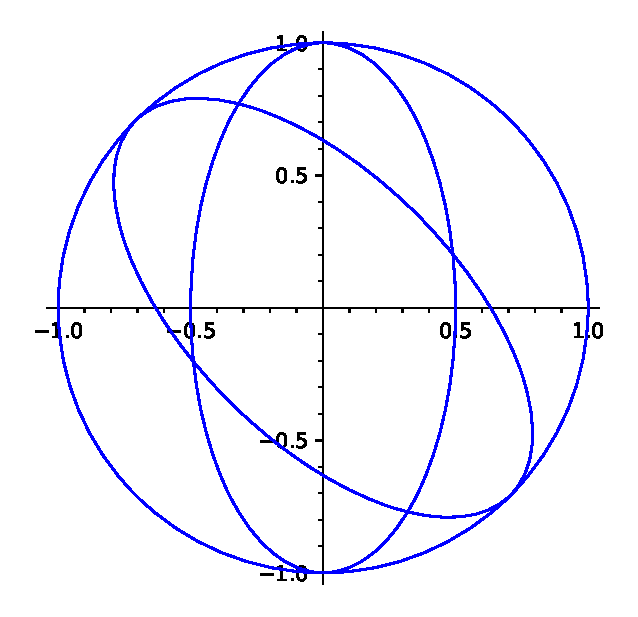
\includegraphics[scale = 0.5]{protbar.eps}
	\end{center}
	\end{figure}
	Abbiamo quindi che per $\mathcal R = \{R_{0}, R_{1}\}$ la norma euclidea standard è estrema, ma non è di Protasov perché ovviamente l'inviluppo convesso delle due ellissi non dà tutto il cerchio e non è nemmeno di Barabanov (si consideri ad esempio il punto $(1,0)$).
	
	Il punto $(3)$ segue dal formalismo della dualità, così come la prima equivalenza del punto $(4)$. Dimostriamo l'ultima equivalenza. $(\Rightarrow)$ che la norma sia estrema segue dal punto $(1)$. Sia ora $v\in\partial C$. Allora $\|v\| = 1$ e per definizione di norma di Barabanov esiste $R\in\mathcal R$ con $\tilde\rho^{-1}\|Rv\| = 1$, ma questo vuol dire che $\tilde\rho^{-1}Rv\in\partial C$. 
	$(\Leftarrow)$ Sia ora $v$ qualsiasi. Senza perdita di generalità, a meno di normalizzarlo possiamo supporre che valga $\|v\| = 1$. Vogliamo quindi dimostrare che $1 = \bigvee_{R\in\mathcal R}\tilde\rho^{-1}\|Rv\|$. Usando l'estremalità della norma abbiamo che
	$$\forall R\in\mathcal R,\; \tilde\rho^{-1}\|Rv\|\leq\tilde\rho^{-1}\|R\|\underbrace{\|v\|}_{=1} \leq \tilde\rho^{-1}\tilde\rho = 1.$$
	Per la disuguaglianza opposta, basta osservare che per la $R$ data dalla condizione si ha $\tilde\rho^{-1}\|Rv\| = 1$, quindi il sup deve essere almeno tale valore.
\end{proof}

\begin{osservazione}
	Nel punto $(4)$ non si chiede che $R$ sia invertibile. In effetti quanto detto funziona con le seminorme, ossia quelle per cui $\|v\|=0$ non implica $v = 0$. L'unica differenza è che in luogo dei CCB assorbenti si usano dei chiusi centrati assorbenti. Ad esempio si può considerare come ``corpo'' la striscia infinita $\R\times[-1,1]$. Esso induce la seminorma $\|(x,y)\| = |y|$. A questo punto considerando come $R = \begin{pmatrix}0 & 0 \\ 0 & 1\end{pmatrix}$ e come $C$ la palla unitaria standard (di $\R$, lungo l'asse $y$!), $R^{-1}C$ è proprio la striscia considerata. 
\end{osservazione}


Diamo ora un corollario ad un teorema della sezione precedente.
\begin{corollario}
	Sia $\mathcal R$ irriducibile. Allora esiste una norma di Protasov per $\mathcal R$.
\end{corollario}
\begin{proof}
	A meno di dividere per $\tilde\rho$ possiamo supporre senza perdita di generalità che $\tilde\rho = 1$. 
	Sia $E$ l'autoinsieme dato dal teorema, vediamo che $C = \conv(E)$ è di Protasov. Ovviamente è compatto, convesso e simmetrico. Inoltre, poiché lo span lineare di $E$ è tutto $\R^{n}$, $C$ è pure assorbente, quindi definisce una norma tramite il funzionale di Minkowski. 
	Bisogna verificare che è di Protasov, ossia che $C = \conv(\mathcal R(C))$. Si ha che 
	\begin{align*}
		\conv\left(\bigcup_{R\in\mathcal R}R[C]\right) &= 
		\conv\left(\bigcup_{R\in\mathcal R}R[\conv E]\right) = 
		\conv\left(\bigcup_{R\in\mathcal R}\conv(RE)\right) \overset{*}{=} \\ &= 
		\conv\left(\bigcup_{R\in\mathcal R}RE\right) = 
		\conv(\mathcal R[E]) = 
		\conv(E) = C.
	\end{align*}
	In $*$ basta osservare che un convesso contiene l'unione $A_{1}\cup\dots\cup A_{t}$ se e solo se contiene $\conv A_{1}\cup\dots\cup\conv A_{t}$, e nel passaggio seguente si usa il fatto che $E$ sia un autoinsieme.
\end{proof}

Analizziamo ora cosa succede considerando lo spazio duale $(\R^{n})^{*}$ identificato con $\R^{n}$ tramite $x\mapsto\langle x, -\rangle$ (attenzione: la $x$ di partenza è il funzionale, quella di arrivo il vettore che lo rappresenta). Un elemento del duale è un funzionale lineare $x:(\R^{n}, \|\cdot\|)\to(\R, |\cdot|)$, per cui la sua norma operatoriale, fissato un CCB $C$, è data da 
$$\|x\|^{*} = \max_{v\neq0}\frac{|\langle x, v\rangle|}{\|v\|} = \max_{\|v\|\leq1}|\langle x, v\rangle| = \max\langle x, C\rangle$$
dove nell'ultima espressione possiamo togliere il valore assoluto in quanto $C$ è simmetrico. 
Ha quindi senso definire il duale di un CCB come 
$$C^{*} = \{x: \|x\|^{*} = 1\} = \{x:\langle x, C\rangle \overset{(=)}{\leq} 1\}.$$
Vediamo ora che questa è una ``vera'' dualità.

\begin{proposizione}
	$C^{**} = C$.
\end{proposizione}
\begin{proof}
	Scriviamo per bene cos'è il biduale di un corpo convesso: 
	$$C^{**} = \{v: \langle C^{*}, v\rangle \leq 1\} = \{v:\forall x\in C^{*},\;\langle x,v\rangle\leq1\} = \{v:\forall x(\langle x,C\rangle\leq1\implies\langle x,v\rangle\leq1)\}.$$
	A questo punto $(\supseteq)$ è ovvio perché se $v\in C$ l'implicazione tra parentesi è automaticamente vera, per cui vediamo $(\subseteq)$. Ci occorre innanzitutto fare l'osservazione chiave che ogni CCB in $\R^{n}$ è l'intersezione di tutti i semispazi chiusi che lo contengono. Questo segue dal teorema di Hahn-Banach, che afferma che se $g:\R^{n}\to\R\geq0$ è subadditiva e $W$ è un sottospazio e $f:W\to\R$ è lineare con $|f|\leq g$, allora esiste $\tilde f$ che estende $f$ a tutto $\R^{n}$ ed è ancora dominata da $g$. 
	
	Nel nostro caso andiamo a dimostrare che $v\not\in C\implies v\not\in C^{**}$.
	Preso $v$, consideriamo il sottospazio $W:=\langle v\rangle$ e su di esso definiamo 
	$$f(sv) := s\|v\|,\quad s\in\R$$
	che è lineare, subadditiva e dominata: $|f(sv)|\leq\|sv\|$.
	Abbiamo allora che per H-B esiste $\tilde f$ che estende $f$, e che possiamo pensare come $\tilde f = \langle x, -\rangle$ per un qualche $x$, ancora dominata: $|\langle x, -\rangle|\leq \|-\|$.
	Tale $x$ testimonia che $v\not\in C^{**}$, infatti se $c\in C$ allora $|\langle x, c\rangle|\leq\| c\|\leq 1$ ma $|\langle x, v\rangle| = |f(v)| = \|v\|>1$ in quanto $v\not\in C$.
\end{proof}

Dato un IFS $\mathcal R$, ad esso si associa $\mathcal R^{T} = \{R^{T}:R\in\mathcal R\}$. Valgono allora alcune considerazioni riassunte nel seguente enunciato.
\begin{lemma}
	\begin{enumerate}
		\item $\mathcal R$ è irriducibile se e solo se $\mathcal R^{T}$ è irriducibile;
		\item $R[C]\subseteq C\iff R^{T}[C^{*}]\subseteq C^{*}$;
		\item $(R[C])^{*} = (R^{T})^{-1}[C^{*}]$ (anche se $R$ non è invertibile);
		\item $(\bigvee_{i} C_{i})^{*} = \bigcap_{i} C_{i}^{*}$.
	\end{enumerate}
\end{lemma}
\begin{proof}
	$(1)$ Sia $0<W<\R^{n}$ un sottospazio $\mathcal R$-invariante. Allora $W^{\perp}$ è proprio (ovvio per dimensionalità) e $\mathcal R^{T}$-invariante. Infatti presi $R\in\mathcal R$ e $v\in W^{\perp}$, si ha che 
	$$\forall w\in W,\; \langle R^{T}v, w\rangle = \langle v, Rw\rangle = 0$$
	in quanto $Rw\in W$ per ipotesi. L'altra implicazione si fa scambiando il ruolo di $\mathcal R$ e $\mathcal R^{T}$.
	$(2)$ è ovvio. 
	$(3)$ segue dalla seguente catena di equivalenze: 
	$$x\in(R[C])^{*} \iff \forall c\in C,\,\langle x, Rc\rangle\leq1\iff\forall c\in C,\,\langle R^{T}x, c\rangle\leq1\iff R^{T}x\in C^{*}.$$
	$(4)$ segue da 
	$$x\in\left(\bigvee_{i}C_{i}\right)^{*}\iff \forall v\in\conv\left(\bigcup_{i}C_{i}\right),\,\langle x,v\rangle\leq1\iff\forall v\in\bigcup_{i}C_{i},\,\langle x,v\rangle\leq 1.$$
\end{proof}

La dualità raggiunge il suo culmine nel seguente
\begin{lemma}[di Wirth]
	Sia $\mathcal R$ irriducibile. Allora $C$ è di Protasov [Barabanov] per $\mathcal R$ se e solo se $C^{*}$ è di Barabanov [Protasov] per $\mathcal R^{T}$.
\end{lemma}
\begin{proof}
	Il caso tra parentesi segue dall'altro gratis poiché $C^{**} = C$ e $\mathcal (R^{T})^{T} = \mathcal R$.
	
	Osserviamo che $\tilde\rho(\mathcal R) = \tilde\rho(\mathcal R^{T})$ e dunque senza perdita di generalità a meno di dividere possiamo supporre $\tilde\rho = 1$. Allora $C$ è di Protasov per $\mathcal R$ se e solo se (lemma) $C = \bigvee_{R\in\mathcal R}R[C]$ se e solo se (dualità)
	\begin{align*}
		C^{*} &= 
		\left(\bigvee_{R\in\mathcal R}R[C]\right)^{*} = 
		\bigcap_{R\in\mathcal R}(R[C])^{*} = 
		\bigcap_{R\in\mathcal R}(R^{T})^{-1}(C^{*}) = 
		\bigcap_{R\in\mathcal R^{T}}R^{-1}(C^{*})
	\end{align*}
	se e solo se (lemma) $C^{*}$ è di Barabanov per $\mathcal R^{T}$.
\end{proof}


\section{Trasformazioni frattali}

Siano dati $\mathcal R = \{R_{0},\dots,R_{N-1}\}$ e $\mathcal S = \{S_{0},\dots,S_{N-1}\}$ non necessariamente strettamente contrattivi, però tali per cui il teorema fondamentale degli IFS sia valido (il punto fondamentale è che $\forall\mathbf a\in\Omega$, $\bigcap_{n\geq0}K_{\mathbf a\upharpoonright n} = \{x\}$).

Consideriamo il seguente diagramma:
$$
\begin{tikzcd}
                                   & \Omega \arrow[ldd, "\pi_\mathcal R", two heads] \arrow[rdd, "\pi_\mathcal S", two heads] &              \\
                                   &                                                                    &              \\
K_\mathcal R \arrow[rr, "\varphi"] &                                                                    & K_\mathcal S
\end{tikzcd}
$$
Le due proiezioni sono suriettive per il teorema fondamentale (vale anche se l'IFS non è contrattivo, a patto di avere l'ipotesi fatta sopra). Vogliamo investigare le proprietà di $\varphi$. L'assunzione cruciale è che le fibre di $\pi_{\mathcal R}$ siano più fini di quelle di $\pi_{\mathcal S}$, ossia che 
$$\forall\mathbf a,\mathbf a'\in\Omega,\;\pi_{\mathcal R}(\mathbf a)= \pi_{\mathcal R}(\mathbf a')\implies \pi_{\mathcal S}(\mathbf a)= \pi_{\mathcal S}(\mathbf a').\quad (*)$$

\begin{lemma}
	Se vale $(*)$, allora $\varphi$ è ben definita e continua. Se inoltre $\pi_{\mathcal R}$ e $\pi_{\mathcal S}$ hanno le stesse fibre, allora $\varphi$ è un omeomorfismo.
\end{lemma}
\begin{proof}
	Consideriamo il seguente diagramma: 
	$$
	\begin{tikzcd}
                                              & \Omega \arrow[ldd, "\pi_\mathcal R", two heads] \arrow[rdd, "\pi_\mathcal S", two heads] \arrow[d, "\alpha", two heads] &              \\
                                              & \Omega/\equiv \arrow[ld, "\beta", two heads, tail] \arrow[rd, "\gamma", two heads]                &              \\
K_\mathcal R \arrow[rr, "\varphi", two heads] &                                                                                                   & K_\mathcal S
\end{tikzcd}
	$$
	Abbiamo posto $\equiv$ la relazione di equivalenza indotta dalle fibre di $\pi_{\mathcal R}$: 
	$$\mathbf a\equiv\mathbf a'\iff \pi_{\mathcal R}(\mathbf a) = \pi_{\mathcal R}(\mathbf a').$$
	Allora è evidente che da $(*)$ segue che $\gamma$ è suriettiva. 
	
	Poniamo ora su $\Omega/\equiv$ la topologia finale. (Ricordiamo cos'è: data $(X,\tau)\xrightarrow[]{F} Y$ con $F$ suriettiva, $A\subseteq Y$ è aperto nella topologia finale se e solo se $F^{-1}[A]$ è aperto in $(X,\tau)$.)
	Abbiamo che $\Omega/\equiv$ è compatto in quanto immagine suriettiva di un compatto, e inoltre che $\beta$ è continua.
	Infatti, dato $B\subseteq K_{\mathcal R}$ aperto, abbiamo che vale $\pi_{\mathcal R}^{-1}B = \alpha^{-1}(\beta^{-1}B)$ e $\beta^{-1}B$ è un aperto in $\Omega/\equiv$ per definizione di topologia finale perché $\pi_{\mathcal R}^{-1}B$ lo è in $\Omega$ per continuità di $\pi_{\mathcal R}$.
	Dunque $\beta$ è un omeomorfismo (per un teorema visto quando abbiamo parlato di funzioni proprie) e dire che $\varphi$ è continua equivale a dire che lo è $\gamma$. Questo fatto si dimostra come appena visto per $\beta$, per cui abbiamo finito.
	
	La seconda parte del teorema è ovvia.
\end{proof}

\begin{esempio}[scala del diavolo]
\end{esempio}


\subsection{Frazioni continue e mappa di Farey}

Consideriamo come al solito $\mathcal R = \{R_{0}, \dots, R_{N-1}\}$ per cui valga il teorema fondamentale degli IFS, e supponiamo di avere la seguente situazione.
$$\begin{tikzcd}
\Omega \arrow[r, "s", two heads] \arrow[d, "\pi", two heads] & \Omega \arrow[d, "\pi", two heads] \\
K \arrow[r, "F", dashed]                                     & K                                 
\end{tikzcd}$$
dove $s$ è l'operatore di shift (ossia tronca il primo simbolo della parola infinita).
Allora spesso si può definire $F$ (almeno su qualche sottoinsieme di $K$) in modo che il diagramma commuti. 
Se ciò è possibile, allora l'unico modo è quello tale che 
$$F\upharpoonright K_{a} = R_{a}^{-1}.$$
Infatti, se consideriamo $x = \pi(a\mathbf b) \overset{TF}{=} R_{a}(\pi(\mathbf b))$, abbiamo che 
$$F(x) = F(\pi(a\mathbf b)) = \pi(s(a\mathbf b)) = \pi(\mathbf b) = R_{a}^{-1}(x).$$
I problemi sorgono quando questa $F$ non è ben definita perché per due immagini vale ad esempio $K_{0}\cap K_{1}\neq\emptyset$, come capita con l'IFS dovuto a Farey,\dots.


\section{Gruppo di Möbius e geometria inversiva}

Sia $n\geq1$, definiamo 
$$\Pi^{n}:=\R^{n}\cup\{\infty\} \simeq S^{n}$$
dove l'isomorfismo è naturalmente dato dalla proiezione stereografica. 

Diamo alcune definizioni per $n=2$, ma si possono facilmente estendere a dimensioni arbitrarie. 
L'\emph{inversione di Möbius} rispetto alla retta $\langle y,w\rangle + \text{cost.} =0$ è data da 
$$x\mapsto x' = x - 2\frac{\langle x, w\rangle}{\langle w, w\rangle}w;$$
rispetto al cerchio di centro $w$ e raggio $r$ è definita implicitamente da 
$$\|x'-w\|\|x-w\| = r^{2},$$
ed esplicitamente da 
$$x\mapsto x' = w + \frac{r^{2}}{\|x-w\|^{2}}(x-w);$$
più in generale, per l'inversione rispetto a $S^{n-1}$ in $S^{n}$ si prende il cono tangente a $S^{n}$ in $S^{n-1}$ di vertice $w$ e, preso $x$, si traccia la retta per $x$ e $w$. L'immagine è l'altro punto di intersezione $x'$ di tale retta con $S^{n}$.

\begin{teorema}
	Sia $\Gamma$ la 2-sfera definita da $\|x-v\| = r$ in $\Pi^{3}$. Allora l'inversione $M$ rispetto a $\Gamma$:
	\begin{enumerate}
		\item fissa globalmente i 2-piani per $v$ ed agisce su di essi tramite l'inversione (nel piano) nella 1-sfera di centro $v$ e raggio $r$;
		\item scambia le 2-sfere per $v$ con i 2-piani non per $v$, e ciò avviene tramite proiezione stereografica rispetto a $v$;
		\item scambia le 2-sfere non per $v$ con altre 2-sfere non per $v$;
		\item per $0\leq m\leq 2$, conserva la classe di $m$-sfere e $m$-piani;
		\item è olomorfa (ossia conserva tutti gli angoli non orientati);
		\item distorce le distanze euclidee, ma conserva i birapporti;
		\item[1'.] fissa globalmente le 2-sfere perpendicolari a $\Gamma$ e agisce su di esse tramite inversione nella 1-sfera di intersezione con $\Gamma$.
	\end{enumerate}
\end{teorema}
\begin{proof}
	Il punto $(1)$ è ovvio. 
	D'ora in poi senza perdita di generalità possiamo supporre che $v = 0$, ossia che $\Gamma = \{y:\|y\| = r\}$. L'espressione esplicita dell'inversione diventa quindi $M(x) = \frac{r^{2}}{\|x\|^{2}}x$.
	Ora, l'equazione $$c\|x\|^{2} + \langle x,w\rangle + d = 0$$ descrive sia i 2-piani che le 2-sfere. Più precisamente si tratta di un 2-piano se e solo se $c = 0$; inoltre passa per $v = 0$ se e solo se $d = 0$. 
	Ora, se l'insieme $S$ è definito da tale equazione, vale 
	\begin{align*}
		M[S] &= 
		\{c\|M^{-1}x\|^{2} + \langle M^{-1}x, w\rangle + d = 0\} \\ &= 
		\{c\|Mx\|^{2} + \langle Mx, w\rangle + d = 0\}\\ &=
		\left\{c\left\|\frac{r^{2}x}{\|x\|^{2}}\right\|^{2} + \langle \frac{r^{2}x}{\|x\|^{2}}, w\rangle + d = 0\right\} \\&= 
		\left\{c\frac{r^{4}}{\|x\|^{2}} + \frac{r^{2}}{\|x\|^{2}}\langle x, w\rangle + d= 0\right\}\\ &= 
		\left\{\frac{d}{r^{2}}\|x\|^{2} + \langle x, w\rangle + cr^{2} = 0\right\}
	\end{align*}
	per cui la prima parte di $(2)$ segue da questa espressione. Per quanto riguarda l'azione come proiezione stereografica, bisogna osservare che qualunque retta per $v$ che taglia la sfera taglia anche il piano non per $v$ in un unico punto.
	
	Il punto $(3)$ segue dall'espressione per $M[S]$.
	
	Per quanto riguarda $(1')$, consideriamo una 2-sfera $\Sigma$ perpendicolare a $\Gamma$. Se dimostriamo che $\Sigma$ è fissata globalmente da $M$, l'affermazione segue; infatti la seconda parte è ovvia per definizione di inversione di una 2-sfera rispetto a un cerchio. 
	Supponiamo quindi che $\Sigma$ abbia centro $w$ e raggio $m$. La perpendicolarità $\Sigma\perp\Gamma$ impone, per Pitagora, che $$\|w\|^{2} = r^{2} + m^{2}.$$
	Dunque $\Sigma$ ha equazione $\|x-w\|^{2} = \|w\|^{2}-r^{2}$, che si traduce in 
	$$-\frac{1}{2}\|x\|^{2} + \langle x, w\rangle - \frac{r^{2}}{2} = 0.$$
	Quindi dall'espressione trovata prima segue che 
	\begin{align*}
		M[\Sigma] &= 
		\left\{\frac{-r^{2}/2}{2}\|x\|^{2} + \langle x, w\rangle + \left(-\frac{r^{2}}{2}\right) =0\right\} \\ &=
		\left\{-\frac{1}{2}\|x\|^{2} + \langle x,w\rangle - \frac{r^{2}}{2} = 0\right\} = \Sigma
	\end{align*}
	Il punto $(4)$ è ovvio. Per dimostrare $(5)$ consideriamo $u\neq 0, \infty$ e due vettori nello spazio tangente $v,w\in T_{u}\R^{3}$. Allora $M$ si fattorizza come 
	$$x\xrightarrow[]{Q} \|u\|^{2}\frac{x}{\|x\|^{2}}\xrightarrow[]{D_{\frac{r^{2}}{\|u\|^{2}}}} M(x),$$
	quindi basta verificare che $Q$ conservi gli angoli dato che ovviamente questo vale per la dilatazione. 
	Si può facilmente calcolare la jacobiana di $Q$, che in ogni punto è simmetrica. Inoltre valgono $Q(u) = u$ e $Q^{2} = \text{Id}$, per cui a livello di jacobiane vale 
	$$\text{Id} = J_{Q^{2}, u} = J_{Q, Q(u)}\cdot J_{Q, u} = J_{Q,u}^{2},$$
	quindi usando la simmetria della jacobiana 
	$$\langle J_{Q,u}v, J_{Q,u}w\rangle = \langle J_{Q,u}^{2}v, w\rangle = \langle \text{Id}v, w\rangle = \langle v,w\rangle$$
	cioè $Q$ conserva gli angoli come volevamo.
	
	Infine vediamo $(6)$ considerando la costruzione in figura. 
	\begin{figure}[htbp]
	\begin{center}
	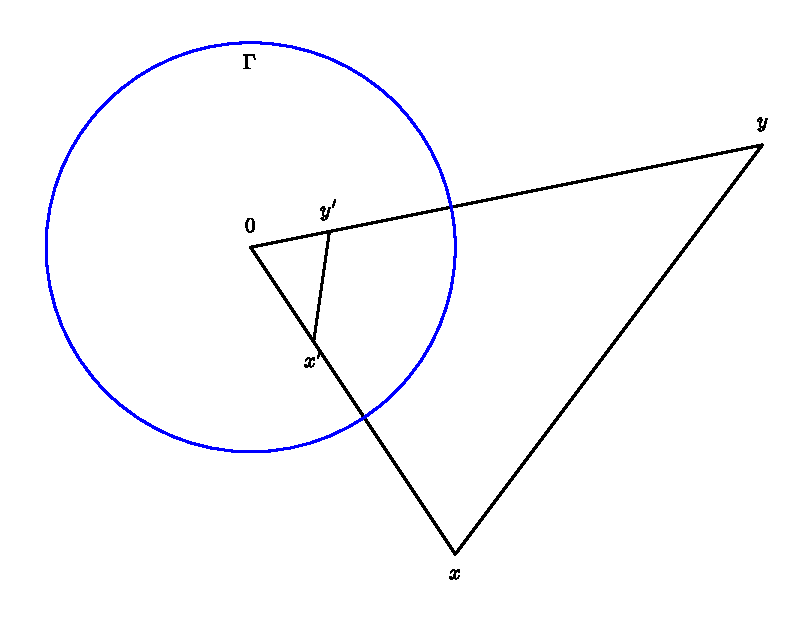
\includegraphics[scale = 0.6]{simili.eps}
	\end{center}
	\end{figure}
	I due triangoli sono simili, avendo un angolo in comune e valendo 
	$$\frac{\|x\|}{\|y'\|} = \frac{\|x\|}{r^{2}/\|y\|} = \frac{\|y\|}{r^{2}/\|x\|} = \frac{\|y\|}{\|x'\|}.$$
	Dunque 
	$$\|x'-y'\| = \|x-y\| \frac{\|y'\|}{\|x\|} = \frac{r^{2}}{\|x\|\|y\|}\|x-y\|,$$
	per cui \emph{in generale} la distanza euclidea non si conserva.
	A questo punto, scegliendo un birapporto (vale per tutti) si trova che
	$$\frac{\|z'-y'\|\|x'-w'\|}{\|z'-x'\|\|y'-w'\|} = \frac{\|z-y\|\frac{r^{2}}{\|z\|\|y\|}\|x-w\|\frac{r^{2}}{\|x\|\|w\|}}{\|z-x\|\frac{r^{2}}{\|z\|\|x\|}\|y-w\|\frac{r^{2}}{\|y\|\|w\|}} = \frac{\|z-y\|\|x-w\|}{\|z-x\|\|y-w\|}.$$
\end{proof}

Ci sono due conseguenze del risultato appena ottenuto. La prima è che dato un \emph{cerchio esteso} (ossia un vero cerchio o una retta) $C$ e un punto $x\not\in C$, l'immagine dell'inversione rispetto a tale cerchio può essere calcolata come l'intersezione della retta che congiunge $x$ con il centro di $C$ con l'unico cerchio (esteso) passante per $x$ e ortogonale a $C$. 
Infatti entrambi i cerchi estesi per $x$ sono fissati globalmente e si intersecano solo in $x$ e $x'$. 

La seconda conseguenza è che la proiezione stereografica coniuga le due definizioni di inversione, quella su $\Sigma^{n}$ e quella su $\Pi^{n}$.

(Fare disegni).

\begin{definizione}
	Dato $n\geq1$ e fissato di conseguenza $S^{n}$ (o equivalentemente $\Pi^{n}$), il \emph{gruppo di Möbius} $\Mob_{n}$ è il gruppo di biezioni di $S^{n}$ generato dalle inversioni nelle $n$-sfere perpendicolari al bordo di $S^{n}$ (o nel caso di $\Pi^{n}$, nelle $(n-1)$-sfere in cui queste intersecano $S^{n}$).
\end{definizione}

\begin{osservazione}
	Il gruppo di Möbius comprende traslazioni, rotazioni, simmetrie assiali e dilatazioni. Pensando in $\Pi^{n}$ è facile capirlo dato che l'inversione rispetto a rette non è altro che la simmetria assiale e con questa si generano rotazioni e traslazioni; le dilatazioni si ottengono invertendo rispetto a due cerchi concentrici.
	Ha un sottogruppo di indice 2, $\Mob_{n}^{+}$, che contiene gli elementi che preservano l'orientazione e si ottiene in modo ovvio moltiplicando un numero pari di elementi di $\Mob_{n}$.
\end{osservazione}

Concentriamoci ora sul caso di $n=2$. 
Dati $z\in\mathbb C\cup\{\infty\}$ e 
$$A=\begin{pmatrix}\alpha & \beta\\\gamma & \delta\end{pmatrix} \in PSL_{2}\mathbb C,$$
l'\emph{omografia indotta da $A$} è la mappa 
$$(A,0)(z) = \frac{\alpha z + \beta}{\gamma z + \delta}$$
mentre l'\emph{antiomografia indotta da $A$} è 
$$(A,1)(z) = \frac{\alpha \bar z + \beta}{\gamma \bar z + \delta}.$$
Risulta evidente che valga il seguente schema per le composizioni di due [anti]omografie:
\begin{align*}
	(A,0)\circ(B,0) &= (AB,0)\\
	(A,0)\circ(B,1) &= (AB,1)\\
	(A,1)\circ(B,0) &= (A\bar B,1)\\
	(A,1)\circ(B,1) &= (A\bar B,0)
\end{align*}
per cui il gruppo di omografie e antiomografie è $PSL_{2}\mathbb C\rtimes \mathbb Z_{2}$.

\begin{osservazione}
	Fissato un cap $\mathcal H^{n}$ di $S^{n}$, sia $\stab(\mathcal H^{n},\Mob_{n})$ il suo stabilizzatore in $\Mob_{n}$. Una volta dimostrato che tale stabilizzatore è generato dalle inversioni rispetto a cerchi perpendicolari al bordo di $\mathcal H^{n}$, dato che queste generano $\Mob_{n-1}$ risulterà $\stab(\mathcal H^{n}, \Mob_{n})\simeq\Mob_{n-1}$.
\end{osservazione}

\begin{lemma}[decomposizione di Iwasawa]
	Ogni $M\in SL_{2}\mathbb C$ è scrivibile in modo unico come $M = KAN$ dove $K \in \mathcal K = SU_{2}\mathbb C$, $A \in \mathcal U = \{\begin{pmatrix}a & 0\\ 0 & a^{-1}\end{pmatrix},\,a>0\}$ e $N\in\mathcal N = \{\begin{pmatrix}1 & \beta\\ 0 & 1\end{pmatrix},\,\beta\in\mathbb C\}$.
\end{lemma}
\begin{proof}
	Consideriamo l'immagine della base canonica tramite $M$, 
	$$(e_{1}, e_{2})M = (m_{1}, m_{2})$$
	e fissato $u_{1} = m_{1}$ imponiamo l'ortogonalità con $u_{2} = m_{2}-\alpha m_{1}$, ossia $\langle m_{1}, m_{2}-\alpha m_{1}\rangle = 0$, che determina $\alpha = \langle m_{1}, m_{2}\rangle /\langle m_{1}, m_{1}\rangle$. Abbiamo quindi la seguente relazione
	$$(u_{1}, u_{2}) = (m_{1},m_{2}) \underbrace{\begin{pmatrix}1 & -\alpha\\ 0 & 1\end{pmatrix}}_{=:N^{-1}}.$$
	La nuova base è ortogonale, quindi poiché 
	$$(e_{1}, e_{2}) MN^{-1} = (u_{1},u_{2})$$
	la matrice $MN^{-1}$ è ortogonale (non per forza hermitiana!). Di conseguenza esiste $a>0$ tale che 
	$$(MN^{-1})^{*}(MN^{-1}) = \begin{pmatrix}a^{2} & 0\\ 0 & a^{-2}\end{pmatrix} =: A^{2}$$
	per cui 
	$$(MN^{-1}A^{-1})^{*}(MN^{-1}A^{-1}) = I_{2}$$
	e quindi $MN^{-1}A^{-1} =: K\in\mathcal K$, e abbiamo dimostrato l'esistenza.
	
	Per quanto riguarda l'unicità della decomposizione, supponiamo che $K_{1}A_{1}N_{1} = K_{2}A_{2}N_{2}$. 
	Allora 
	$$N_{1}^{*}A_{1}^{*}\underbrace{K_{1}^{*}K_{1}}_{=I_{2}}A_{1}N_{1} = N_{2}^{*}A_{2}^{*}\underbrace{K_{2}^{*}K_{2}}_{=I_{2}}A_{2}N_{2}$$
	per cui dal fatto che le $A_{i}$ sono diagonali a elementi reali si ha $A_{i}^{*} = A_{i}$, quindi 
	$$N_{1}^{*}A_{1}^{2}N_{1} = N_{2}^{*}A_{2}^{2}N_{2}.$$
	A questo punto moltiplichiamo a sinistra per $(N_{2}^{*})^{-1}$ e a destra per $N_{1}^{-1}$, ottenendo
	$$(N_{2}^{*})^{-1} N_{1}^{*} A_{1}^{2} = A_{2}^{2} N_{2}N_{1}^{-1}$$
	e qui il termine a sinistra è triangolare inferiore, quello a destra triangolare superiore. Di conseguenza entrambi devono in realtà essere diagonali, da cui seguono $N_{1} = N_{2}$ e $A_{1} = A_{2}$. 
\end{proof}

\begin{teorema}
	Vale $\Mob_{2} = PSL_{2}\mathbb C\rtimes\mathbb Z_{2}$, e di conseguenza $\Mob_{2}^{+} = PSL_{2}\mathbb C$.
\end{teorema}
\begin{proof}
	$(\subseteq)$ L'inversione rispetto alla circonferenza unitaria centrata nell'origine è data da 
	$$z\mapsto \frac{1}{\bar z} = \left(\begin{pmatrix}0 & i\\ i & 0\end{pmatrix}, 1\right)$$
	per cui è un'antiomografia. 
	La dilatazione di un generico fattore $r>0$ è data da 
	$$\left(\begin{pmatrix}r^{1/2} & 0\\ 0 & r^{-1/2}\end{pmatrix}, 0\right),$$
	la traslazione di $\alpha\in\mathbb C$ da 
	$$\left(\begin{pmatrix}1 & \alpha\\ 0 & 1\end{pmatrix}, 0\right)$$
	e quindi per le inversioni rispetto a cerchi va tutto bene. 
	Per quanto riguarda le inversioni rispetto a rette, sono tutte coniugate (a meno di rototraslazione) a quella rispetto all'asse reale, e questa è indotta da 
	$$\left(\begin{pmatrix}1 & 0\\ 0 & 1\end{pmatrix}, 1\right).$$
	
	$(\supseteq)$ Si utilizza la decomposizione di Iwasawa per elementi di $SL_{2}\mathbb C$, per cui preso un generico $M\in SL_{2}\mathbb C$ abbiamo $M = KAN$. Abbiamo che $A,N\in \Mob_{2}$, per cui ci resta da determinarlo per $K\in SU_{2}\mathbb C$.
	Studiamo meglio la forma di $K = \begin{pmatrix}\alpha & \beta \\\gamma & \delta\end{pmatrix}$.
	Dato che sta in $SU_{2}\mathbb C$, deve valere $K^{-1} = K^{*}$ che si traduce in termini di elementi come $\delta = \bar\alpha$ e $\gamma = -\bar\beta$, per cui abbiamo che 
	$$\begin{pmatrix}\alpha & \beta \\ -\bar\beta & \bar\alpha\end{pmatrix},\quad \det K = |\alpha|^{2} + |\beta|^{2} = 1.$$
	Se $K\neq\pm \text{Id}$, ci sono due autovalori complessi coniugati di modulo 1 e due corrispondenti autovettori. 
	
	Osserviamo ora che $\forall p,q\in P^{1}\mathbb C$ esiste un elemento $B$ di $\Mob_{2}$ che manda $p\mapsto\infty$ e $q\mapsto1$. Infatti se $p=\infty$ basta applicare una traslazione, se $p\neq\infty$ si considera l'inversione rispetto alla circonferenza di centro $p$ e passante per $q$ e si ricade nel caso procedente.
	
	Possiamo quindi supporre senza perdita di generalità che gli autovettori di $K$ siano $1$ e $\infty$. L'equazione che testimonia questo fatto è 
	$$BKB^{-1}\begin{pmatrix}1 & 0\\ 0& 1\end{pmatrix} = \begin{pmatrix}\rho & 0\\ 0& \bar\rho\end{pmatrix}\begin{pmatrix}1 & 0\\ 0& 1\end{pmatrix} $$
	e osserviamo che la penultima matrice è una rotazione di angolo $2\text{arg}(\rho)$, che sta in $\Mob_{2}$. Quindi $K\in\Mob_{2}$.
\end{proof}

Lo spazio iperbolico $\mathcal H^{3}$ si può pensare in due modi: come l'interno di una sfera $S^{2}$ (che sarebbe un cap di $S^{3}$) oppure grazie alla proiezione stereografica come la parte ``sopra'' al piano $\mathbb C\cup\{\infty\}$. 
La distanza che si usa è quella iperbolica, definita inizialmente per il modello di Klein di $\mathcal H^{2}$ ma che va bene anche per gli altri casi, data da 
$$d_{B}(p_{1}, p_{2}) = \log\frac{\|p_{0} - p_{2}\|\|p_{1} - p_{3}\|}{\|p_{0} - p_{1}\|\|p_{2} - p_{3}\|}$$
dove $p_{0}$ e $p_{3}$ sono i punti che si ottengono facendo l'intersezione dell'unico $1$-cerchio per $p_{1}$ e $p_{2}$ perpendicolare a $\partial \mathcal H^{2}$ (o $\partial \mathcal H^{3}$) con tale bordo. 
Poiché le inversioni conservano il birapporto, gli elementi di $\Mob_{2}$ (o $\Mob_{3}$) sono isometrie per lo spazio iperbolico. Precisiamo questo fatto nel seguente teorema.

\begin{teorema}
	Ogni isometria di $\mathcal H^{3}$ è nel sottogruppo di $\Mob_{3}$ generato dalle inversioni nelle 2-sfere perpendicolari a $\partial\mathcal H^{3}$ (più in generale per il caso di $\mathcal H^{n}$ bastano $n+1$ inversioni). In particolare, tale sottogruppo è proprio $\stab (\mathcal H^{3}, \Mob_{3})$.
\end{teorema}
\begin{proof}[Schema di dimostrazione]
	Per omogeneità, un'isometria è determinata dalla sua azione su un qualsiasi simplesso dello spazio. 
	Preso dunque un tetraedro di vertici $p_{0}, p_{1}, p_{2}, p_{3}$ e un'isometria $\Phi$, diciamo che le immagini dei vertici del tetraedro siano $q_{0}, q_{1}, q_{2}, q_{3}$. 
	Si manda dunque $p_{0}\mapsto q_{0}$ con un'opportuna inversione (questo è facile!). 
	Dopodiché si prende un'inversione che manda $p_{1}\mapsto q_{1}$ ma la cui sfera contiene $q_{0}$, che quindi resta fissato, e così avanti. 
	Si riesce giusto in tempo perché c'è solo una sfera per tre punti e perpendicolare al bordo, ma è proprio quella che scambia tra loro i due possibili tetraedri costruiti sulle immagini dei primi tre punti.
\end{proof}

$$
\begin{tikzcd}[cramped, column sep = small]
                                             & \Mob_3 \arrow[d, no head]                                                                                                               &                                                                    \\
                                             & PSL_2\mathbb C\rtimes\mathbb Z_2 = \Mob_2 = \stab\mathcal H^3 = \text{Iso}^\pm\mathcal H^3 \arrow[ld, "2", no head] \arrow[rd, no head] &                                                                    \\
PSL_2\mathbb C = \Mob_2^+ \arrow[rd, "(**)", no head] &                                                                                                                                        & \Mob_1 = \stab\mathcal H^2 = PSL_2\mathbb R\rtimes\mathbb Z_{2} \arrow[ld, "(*)", no head] \\
                                             & \Mob_1^+ = PSL_2\mathbb R                                                                                                               &                                                                   
\end{tikzcd}
$$

\begin{osservazione}
	Consideriamo un generico $z\in\mathbb C$. Esso appartiene a $\mathcal H^{2}$ se e solo se 
	$$\begin{pmatrix}z \\ 1\end{pmatrix}^{*} \begin{pmatrix}0 & -i \\ i & 0\end{pmatrix} \begin{pmatrix}z \\ 1\end{pmatrix}<0.$$
	Infatti svolgendo i conti si ottiene che tale condizione equivale a 
	$$-i\bar z + iz = i(z-\bar z) = i2\Im z\cdot i = -2\Im z < 0.$$
	Ne segue che una generica matrice $A = \begin{pmatrix}\alpha & \beta \\ \gamma & \delta\end{pmatrix}\in PSL_{2}\mathbb C$ stabilizza globalmente il piano iperbolico $\mathcal H^{2}$ (considerato nel modello del semipiano) se e solo se lascia invariata tale forma, ossia 
	$$A^{*}\begin{pmatrix}0 & -i \\ i & 0\end{pmatrix}A = \begin{pmatrix}0 & -i \\ i & 0\end{pmatrix}.$$
	(In realtà questa relazione dovrebbe valere a meno di costante moltiplicativa perché quello che ci interessa è soltanto che il segno della forma resti invariato, ma la costante moltiplicativa si può sempre assorbire nella matrice di $PSL_{2}\mathbb C$).
	Svolgendo i calcoli si ottiene che ciò equivale a $\alpha, \beta,\gamma,\delta\in\R$, che dimostra $(**)$ nel reticolo qui sopra.
	
	Per tornare al piano di sopra dall'altro lato $(*)$, bisogna aggiungere l'inversione $z\mapsto -\bar z$, che è indotta da 
	$$\left(\begin{pmatrix}i & 0 \\ 0 & i^{-1}\end{pmatrix}, 1\right)$$
	ma anche da 
	$$\left(\begin{pmatrix}-1 & 0 \\ 0 & 1\end{pmatrix}, 1\right)$$
	che è una scelta più furba perché permette di non uscire dai reali.
\end{osservazione}

\subsection{Gruppi fuchsiani/kleiniani}

\begin{lemma}
	Sia $\mathcal G$ un gruppo che agisce in modo transitivo sullo spazio topologico di Hausdorff localmente compatto $X$. Le due condizioni seguenti sono equivalenti e definiscono un'\emph{azione propriamente discontinua}:
	\begin{enumerate}
		\item $\forall x\in X,\;\forall K\subseteq X$ compatto, $\#\{G\in\mathcal G:\,Gx\in K\}<\infty$;
		\item l'orbita di ogni $x\in X$ è discreta e ogni punto ha stabilizzatore finito. 
	\end{enumerate}
\end{lemma}
\begin{proof}
	$(1\implies 2)$ Che lo stabilizzatore sia finito si ottiene facilmente scegliendo $K = \{x\}$. 
	Ora, visto che l'azione è transitiva, basta dimostrare che $\forall x\in X,\,\exists O\ni x$ aperto con $O\cap \mathcal G*x = \{x\}$.
	Per la locale compattezza, questo $O$ si può scegliere in modo che la sua chiusura sia compatta. Per $(1)$ però questo implica che tale chiusura contenga un numero finito di punti dell'orbita. Quindi qui fissato un particolare punto dell'orbita, esso si può separare dagli altri grazie all'ipotesi che lo spazio sia di Hausdorff. 
	
	$(2\implies1)$ Dati $x$ e $K$, per ipotesi abbiamo che $\mathcal G*x$ è discreta. Poiché $K$ è compatto, l'intersezione $\mathcal G*x\cap K$ è finita. Infine la cardinalità dell'insieme delle mappe da $x$ a un certo $y$ è la stessa dello stabilizzatore di $y$, che per ipotesi è finito. Di conseguenza è finita anche la cardinalità dell'insieme delle mappe che mandano $x$ nei punti di $\mathcal G*x\cap K$, in quanto unione finita di insiemi finiti.
\end{proof}

\begin{osservazione}
	Se $\mathcal G$ è anche un gruppo topologico e l'azione è continua e propria (cioè i controinsiemi di compatti sono compatti, rispetto alla mappa $G\times X\to X$) e consideriamo un sottogruppo $\Gamma\leq\mathcal G$ discreto, allora l'azione di $\Gamma$ su $X$ è propriamente discontinua. 
\end{osservazione}
\begin{proof}
	Verifichiamo la condizione 1 del lemma, ossia che dati $x$ e $K$, l'insieme $\{G\in\Gamma:\, Gx\in K\}$ è finito. 
	Tale insieme si può riscrivere come 
	$$\Gamma\cap \{G\in\mathcal G:\, Gx\in K\} = \Gamma \cap \{(G,y)\in\mathcal G\times X:\,Gy\in K\}\cap \pi^{-1}\{x\}$$
	e siccome l'azione è propria, $\{(G,y):\,Gy\in K\}$ è compatto; inoltre $\pi^{-1}\{x\}$ è chiuso, per cui anche l'intersezione $\{(G,y):\,Gy\in K\}\cap \pi^{-1}\{x\}$ è compatta essendo un chiuso in un compatto. Infine, essendo $\Gamma$ discreto, ovviamente intersecandolo con un compatto si ottiene un insieme finito.
\end{proof}

\begin{definizione}
	Un sottogruppo $\Gamma$ di $\Mob_{n-1}$ che agisce in modo propriamente discontinuo su $\mathcal H^{n}$ si dice un \emph{gruppo fuchsiano esteso} se $n=2$ (ossia è un sottogruppo di $PSL_{2}\R\rtimes\mathbb Z_{2}$), un \emph{gruppo kleiniano esteso} se $n=3$ (sottogruppo di $PSL_{2}\mathbb C\rtimes\mathbb Z_{2}$). I loro sottogruppi che preservano l'orientazione si dicono \emph{gruppi fuchsiani} e \emph{kleiniani} rispettivamente. 
\end{definizione}

\begin{esempio}
	$PSL_{2}\mathbb Z$ e $PSL_{2}\mathbb Z\rtimes\mathbb Z_{2}$ sono fuchsiani; il gruppo modulare di Picard $PSL_{2}\mathbb Z[i]$ è kleiniano. Esempi più generali si hanno considerando i vari $PSL_{2}\mathbb O$, dove $\mathbb O$ è l'anello degli interi algebrici di una fissata estensione quadratica complessa di $\mathbb Q$, detti gruppi di Bianchi.
	Le estensioni quadratiche \emph{reali} non vanno bene, perché se ad esempio abbiamo $\mathbb Q(\lambda)$ di grado 2, vale 
	$$
	\begin{pmatrix}
	1 & \lambda^{-k}\\
	0 & 1
	\end{pmatrix}
	\xrightarrow[]{k\to\infty}
	\begin{pmatrix}
	1 & 0\\
	0 & 1
	\end{pmatrix}$$
	quindi l'identità $I_{2}$ è punto di accumulazione, per cui non si possono avere orbite discrete.
\end{esempio}

\subsection{Classificazione inversioni}

Abbiamo visto che i gruppi $\text{Mob}_1^+$ e $\text{Mob}_2^+$ sono isomorfi a $PSL_2\mathbb R$ e $PSL_2 \mathbb C$ rispettivamente. 
Vogliamo classificare le trasformazioni di tali gruppi, e lo facciamo per il più grande (la classificazione delle trasformazioni di $PSL_2\mathbb R$ sarà una conseguenza di questa).

Consideriamo quindi una generica matrice 
$$A = \begin{pmatrix}\alpha & \beta \\ \gamma & \delta\end{pmatrix}\in PSL_2\mathbb C.$$
Essa agisce in modo naturale su $P^1\mathbb C$ e per estensione anche su $\mathcal H^3$ pensato come lo spazio "sopra" a $P^1\mathbb C$.

\begin{osservazione}
In effetti possiamo pensare ad $\mathcal H^3$ come ad un sottoinsieme dei quaternioni $\mathbb H$, in particolare quello dei quaternioni della forma 
$$q = z + rj,\quad z\in\mathbb C,\, r>0.$$
A questo punto l'inversione rispetto ad una circonferenza di $P^1\mathbb C$ agisce su $\mathcal H^3$ come l'inversione rispetto alla (unica) sfera che ha tale circonferenza come equatore. 
Algebricamente, ricordando che i quaternioni non sono commutativi, l'azione della matrice $A$ definita sopra si esprime come 
$$A*q = (\alpha q + \beta)(\gamma q + \delta)^{-1}.$$
\end{osservazione}

Vediamo che la classificazione di tali trasformazioni dipende essenzialmente dalla traccia della matrice, $t := \alpha + \delta$.
Essendo il polinomio caratteristico dato da $x^2 - tx + 1$, gli autovalori di $A$ sono $\frac{t\pm\sqrt{t^2 - 4}}{2}$. Distinguiamo alcuni casi.
\begin{itemize}
    \item $t^2 = 4$, ovvero $t = \pm2$. Abbiamo allora un unico autovalore che vale $\pm1$ e $A$ risulta coniugata a 
    $$\begin{pmatrix}1 & 1\\0 & 1\end{pmatrix}$$
    che (sul piano) agisce come una traslazione euclidea. $A$ in questo caso si dice \emph{parabolica}.
    \item $t\in(-2, 2)\subset\mathbb R$. Allora gli autovalori sono $\rho$ e $\bar\rho$ e la matrice $A$ è coniugata a 
    $$\begin{pmatrix}\rho & 0\\0 & \bar\rho\end{pmatrix}$$
    che agisce sul piano come una rotazione $z\mapsto \rho^2 z$. 
    $A$ si dice \emph{ellittica}.
    \item $t\in\mathbb C\setminus [-2,2]$. Allora gli autovalori sono $\rho$ e $\rho^{-1}$ con $|\rho|>1$, $A$ è coniugata a 
    $$\begin{pmatrix}\rho & 0\\0 & \rho^{-1}\end{pmatrix}$$
    e agisce come una rotodilatazione $z\mapsto\rho^2 z$. $A$ si dice \emph{lossodromica}.
    Un sottocaso particolare di questo si ha quando $t\in\mathbb R\setminus [-2,2]$, nel qual caso $A$ si dice \emph{iperbolica} (e infatti per le matrici di $PSL_2\mathbb R$ di solito si parla solo di queste ultime).
\end{itemize}

\subsection{Insiemi limite}
\begin{definizione}
    Sia $\Gamma<PSL_2\mathbb C$ kleiniano. Il suo \emph{insieme limite} è 
    $$\Lambda = \Lambda(\Gamma) = \{p\in\partial\mathcal H^3:\; 
    \exists q\in\mathcal H^3 \text{ t.c. $p$ è di accumulazione per l'orbita $\Gamma*q$ di $q$}\}.$$
\end{definizione}

Importante: nella definizione appena data, l'accumulazione si intende rispetto alla norma euclidea. 

\begin{osservazione}
    Se $p$ è di accumulazione per $\Gamma*q$, allora lo è pure per $\Gamma*t$.
\end{osservazione}
\begin{proof}
    Se $p$ è di accumulazione per $\Gamma*q$, allora esiste una successione $G_0,G_1,\dots\in\Gamma$ tale che $G_n*q\to p$ in senso euclideo per $n\to\infty$.
    Consideriamo l'orbita $G_n*t$. Poiché le $G_n$ stanno in $PSL_2\mathbb C$, esse conservano la distanza iperbolica. Quindi se $d$ è la distanza iperbolica tra $q$ e $t$, è anche la distanza iperbolica tra $G_n q$ e $G_n t$ per ogni $n$. Però siccome il punto di accumulazione $p$ di $\Gamma*q$ sta sul bordo $\partial\mathcal H^3$, tali distanze in senso euclideo vanno a 0, per cui si può concludere per la disuguaglianza triangolare che $G_n * t\to p$.
\end{proof}

\begin{osservazione}
    Ovviamente $\Lambda$ è un chiuso perché il suo complementare $\Omega = \partial\mathcal H^3\setminus \Lambda$, detto anche \emph{insieme regolare} o \emph{dominio di discontinuità} di $\Gamma$ è aperto. 
    Altrettanto ovviamente $\Lambda$ è $\Gamma$-invariante, e gli elementi di $\Gamma$ agiscono su $\Lambda$ come omeomorfismi.
    Una proprietà meno ovvia è che se $\Lambda$ non ricade in alcuni casi speciali (vuoto, un punto, due punti, $\partial\mathcal H^{3}$) allora è un \emph{perfetto} (chiuso senza punti di accumulazione) ad interno vuoto.
\end{osservazione}
\begin{esempio}
	Le rotazioni non hanno punti di accumulazione sul bordo; le lossodromiche ne hanno due; il gruppo di inversioni generato da quelle in cerchi con diametri tutti lungo una circonferenza massima di $\partial \mathcal H^{3}$ ha come insieme limite la circonferenza massima stessa; il gruppo di Picard ha (probabilmente) $\Lambda = \partial \mathcal H^{3}$.
\end{esempio}


\subsection{Unificazione di cap e punti}

Consideriamo ora il gruppo (fuchsiano esteso) generato dalle inversioni rispetto a tre cerchi disgiunti in $P_1\mathbb C$ (o in alternativa in $S^{2}$).
Vogliamo studiare il suo comportamento utilizzando il chaos game. 
Siccome le trasformazioni che andiamo ad applicare sono involuzioni, è importante non applicare due volte consecutive la stessa. Questo obiettivo si può raggiungere facilmente se l'indice della "nuova" trasformazione da applicare si ottiene sommando 1 o 2 e poi facendo mod 3.

Se usassimo un gruppo fuchsiano tipo 
$$\Gamma = \langle A_0, \dots, A_{N-1}, A_0^{-1},\dots, A_{N-1}^{-1}\rangle$$
avremmo il problema simile di evitare di applicare una trasformazione e la sua inversa consecutivamente. 

Vediamo ora una interessante costruzione che permette di rendere tutto più semplice. 
Consideriamo la sfera $S^n$. Ad un suo cap $C$ si può associare il suo centro $c\in S^n$ e l'angolo di apertura $\theta\in(0,\pi)$.
Allora il cap si può caratterizzare come 
\begin{align*}
    C &= \{x\in S^n:\; \langle x, c\rangle \geq\cos\theta\} = 
    \{x\in S^n:\; \langle x, c\rangle -\cos\theta\geq 0\} \\&= 
    \{x\in S^n:\; \langle x, \frac{c}{\sin\theta}\rangle - \cot\theta\geq 0\}.
\end{align*}
A questo punto descriviamo sia i punti che i caps come dei vettori in $\mathbb R^{n+2}$ tramite le seguenti associazioni: 
\begin{itemize}
    \item $x\in S^n$ viene associato a $\mathbf{x} = (x_1,\dots,x_{n+1}, 1)^t$;
    \item $C\sim(c,\theta)$ viene associato a $\mathbf{w} = (c_1/\sin\theta,\dots,c_{n+1}/\sin\theta, \cot\theta)^t$.
\end{itemize}
D'ora in avanti useremo $\langle-,-\rangle$ anche per vettori in $\mathbb R^{n+2}$ indicando il prodotto scalare di Lorentz di segnatura $(n+1,1)$. Dal contesto (vettori in grassetto) sarà sempre chiaro quale stiamo usando. 

Con queste convenzioni, abbiamo le seguenti conseguenze: 
\begin{itemize}
    \item $x\in C$ se e solo se $\langle \mathbf{x}, \mathbf{w}\rangle \geq0$;
    \item $\mathbf x\in\mathbb R^{n+2}$ corrisponde ad un punto se e solo se $\mathbf x_{n+1} = 1$ e $\langle\mathbf{x}, \mathbf{x}\rangle = 0$;
    \item $\mathbf{w}\in\mathbb R^{n+2}$ corrisponde ad un cap se e solo se appartiene allo \emph{spazio di De Sitter} $S= \{\mathbf z\in\mathbb R^{n+2}:\;\langle\mathbf{z}, \mathbf{z}\rangle = 1\}$.
\end{itemize}
\begin{proof}
    Dimostriamo solo l'ultima equivalenza. $(\Rightarrow)$ è immediato: 
    $$\left(\frac{c_1}{\sin\theta}\right)^2+\dots + \left(\frac{c_{n+1}}{\sin\theta}\right)^2 - (\cot\theta)^2 = \frac{1-(\cos\theta)^2}{(\sin\theta)^2} = 1.$$
    Vediamo $(\Leftarrow)$. Sia $\mathbf y$ tale che $\langle\mathbf{y}, \mathbf{y}\rangle = 1$. Basta porre $\theta = \text{arccot} y_{n+2}$ e di conseguenza, dato che il centro del cap deve appartenere alla sfera, $c:=(y_1,\dots,y_{n+1})/(1 + y_{n+2}^2)^{1/2}$.
\end{proof}

La magia di tutta questa costruzione sta nel seguente risultato. 
\begin{teorema}
L'inversione rispetto a $C\sim \mathbf w$ è data da 
$$\mathbf x\mapsto\mathbf x - 2\langle\mathbf{w}, \mathbf{x}\rangle\cdot\mathbf w$$
\end{teorema}

Tale mappa se consideriamo come ambiente $S^2$ è un elemento di $GL_4\mathbb R$, più precisamente di $O_{3,1} \mathbb R$. La cosa importante è che possiamo scriverla in modo esplicito(!), infatti preso un punto $\mathbf x = (x_1,x_2, x_3, 1)^t$ la sua immagine è 
$$I\mathbf x - 2 \mathbf w\mathbf w^t\begin{pmatrix}1 & & & \\ & 1 & & \\ & & 1 & \\ & & & -1\end{pmatrix}\mathbf x = [I - 2 \mathbf w\mathbf w^t L]\mathbf x.$$

Esercizio in SageMath: consideriamo inizialmente i tre cap corrispondenti a $\mathbf w_0 = (0, 1, -1, 1)^t$, $\mathbf w_1 = (0, -1, -1, 1)^t$, $\mathbf w_0 = (0, -1, 1, 1)^t$ e usiamo il chaos game su questi. Infine aggiungiamo un cap parametrico $\mathbf w_4 = (1/\sin\theta, 0, 0, \cot\theta)$ e facciamo variare $\theta$ facendolo crescere fino a quando il cap corrispondente non è tangente agli altri tre.  


\begin{teorema}
	L'inversione nel cap $C\sim \mathbf w$ è data dalla mappa
	$$\mathbf x\mapsto\mathbf x - 2 \frac{\langle \mathbf w, \mathbf x\rangle}{\langle \mathbf w, \mathbf w\rangle}\mathbf w.$$
	Tale mappa è un elemento di $O_{3,1}\R$, e tale espressione funziona sia per i punti che per i cap.
\end{teorema}
\begin{proof}
	Dati $S^{3}$ e $\mathbf w$, osserviamo che $\langle \mathbf x,\mathbf w\rangle = 0$ individua il piano polare a $\mathbf w$ rispetto alla conica $S^{3}$. 
	Allora preso un generico $\mathbf x$, possiamo scriverlo in modo unico come $\mathbf x = \mathbf u + r\mathbf w$ con $\mathbf u$ in tale piano polare. La sua immagine tramite la mappa definita nell'enunciato è $\mathbf x' = \mathbf u-r\mathbf w$. 
	Osserviamo che $\mathbf x\mapsto\mathbf x'$ conserva la forma di Lorentz (esercizio), per cui se dimostriamo che i tre punti $x,x',w$ (corrispondenti nello spazio di partenza di $\mathbf x,\mathbf x'$, con l'ultimo che è il ``vertice'' del cap corrispondente a $\mathbf w$) sono allineati allora $x'$ è proprio l'immagine di $x$ tramite l'inversione nel cap $C_{\mathbf w}$, in quanto valgono $\langle \mathbf x',\mathbf x'\rangle = \langle \mathbf x,\mathbf x\rangle = 0$ e l'intersezione di una retta con $S^{2}$ ha due punti (ricordare la costruzione geometrica dell'inversione!). 
	Che siano allineati si ottiene considerando il fatto che $\mathbf x' = \mathbf x - 2 \frac{\langle \mathbf w, \mathbf x\rangle}{\langle \mathbf w, \mathbf w\rangle}\mathbf w$, per cui $\mathbf x',\mathbf x,\mathbf w$ stanno sullo stesso 2-piano e quindi $x,x',w$ sulla stessa retta proiettiva.
	
	La stessa formula funziona anche per i cap perché conserva la forma di Lorentz e quindi manda cap in cap. Inoltre, per lo stesso motivo, manda $\mathbf x\in C_{\mathbf w}$ in $\mathbf x'\in C_{\mathbf w'}$, dato che l'appartenenza ad un cap si esprime in termini di forma di Lorentz.
\end{proof}


\begin{lemma}
	Sia $A\in O_{3,1}\R$. Allora $a_{44}\neq0$ e $A$ fissa globalmente ognuna delle due componenti connesse $\pm\mathcal L$ di $\{\mathbf x:\langle \mathbf x,\mathbf x\rangle = -1\}$ oppure le scambia a seconda del segno di $a_{44}$.
	Di conseguenza l'omomorfismo 
	$$O_{3,1}\R\to\mathbb Z_{2}\times\mathbb Z_{2},\quad A\mapsto(\det A, \text{sgn}a_{44})$$
	induce l'affettamento di $O_{3,1}\R$ in
	$$\begin{matrix}
	   & \text{sgn}=1 & -1\\
	 \det = 1 & SO_{3,1}^{\uparrow}\R & \begin{pmatrix}1 & & & \\ & -1 & & \\ & & 1 & \\ & & & -1\end{pmatrix}SO_{3,1}^{\uparrow}\R\\
	 -1 & \begin{pmatrix}1 & & & \\ & -1 & & \\ & & 1 & \\ & & & 1\end{pmatrix}SO_{3,1}^{\uparrow}\R & \begin{pmatrix}1 & & & \\ & 1 & & \\ & & 1 & \\ & & & -1\end{pmatrix}SO_{3,1}^{\uparrow}\R
	\end{matrix}$$ 
	con la prima riga che forma tutto $SO_{3,1}\R$ e la prima colonna che forma $O_{3,1}^{\uparrow}\R$. La freccia in su indica che il gruppo non scambia $\pm\mathcal L$.
\end{lemma}
\begin{proof}
	Siano $\mathbf v = (0,0,0,1)^{t}\in\mathcal L$ e $A\in O_{3,1}$. 
	Per definizione la forma di Lorentz viene conservata da $A$, per cui vale 
	$$-1 = \langle \mathbf v,\mathbf v\rangle = \langle A\mathbf v, A\mathbf v\rangle = a_{14}^{2} + a_{24}^{2} + a_{34}^{2}-a_{44}^{2}$$
	e quindi necessariamente deve essere $a_{44}\neq0$.
	
	Infine per vedere se le due componenti $\pm\mathcal L$ vengono scambiate o meno basta (per connessione e continuità) vedere in quale delle due falde sta l'immagine di $\mathbf v$, ossia valutare la sua quarta coordinata $a_{44}$. La tesi è a questo punto ovvia.
\end{proof}


\begin{teorema}
	La mappa che ad ogni inversione in $P^{1}\mathbb C$ rispetto al cap $C\sim \mathbf w$ associa la matrice $R_{\mathbf w}\in O_{3,1}\R$ che induce la trasformazione del Teorema 53, esplicitamente data da $R_{\mathbf w} = I-2\mathbf w\mathbf w^{t}L$ induce due isomorfismi
	$$PSL_{2}\mathbb C\to SO_{3,1}^{\uparrow}\R,\quad PSL_{2}\mathbb C\rtimes\mathbb Z_{2}\to O_{3,1}^{\uparrow}\R.$$
\end{teorema}
\begin{proof}
	Per prima cosa osserviamo che per il teorema precedente la matrice $R_{\mathbf w}$ preserva $\mathcal L$ in quanto $(R_{\mathbf w})_{4,4} = 1-2w_{4}^{2}\cdot(-1) = 1+2w_{4}^{2}>0$.

	Che la mappa descritta induca omomorfismi è ovvio.
	Abbiamo che l'inversione $(I,1): z\mapsto \bar z$ corrisponde a $R_{\mathbf e_{2}}$: è l'inversione rispetto al cerchio massimo di $S^{2}$ ``parallelo all'asse reale''.
	Per dimostrare che l'omomorfismo è iniettivo supponiamo per assurdo che $(A,0/1)\mapsto I_{\R^{4}}$. Allora l'immagine in particolare fissa globalmente $\{\mathbf x:\langle\mathbf x,\mathbf x\rangle = 0\} = S^{2}$ per cui in particolare $A = \pm I$ e, dato che nessuna antiomotetia è l'identità su $S^{2}$, deve essere $A = I$.
	
	Infine resta da verificare la suriettività. 
	Facciamo un giro un po' lunghetto. Consideriamo $\mathfrak w := \{W\in \mathbb C^{2\times 2}:\, W^{*} = -W\} = \mathfrak u_{2}\mathbb C$. Facendo i conti si scopre che le matrici di $\mathfrak w$ hanno la forma
	$$
	W = \begin{pmatrix}
	ri & \beta\\
	-\bar\beta & si
	\end{pmatrix},
	\quad \beta\in\mathbb C,\; r,s\in\R$$
	per cui abbiamo quattro gradi di libertà (reali).
	
	Ora consideriamo la seguente operazione: prendiamo $A\in PSL_{2}\mathbb C$ e coniughiamo $W$ per $A^{-1}$. Allora si rimane in $\mathfrak w$, infatti 
	$$[(A^{-1})^{*}WA^{-1}]^{*} = (A^{-1})^{*}W^{*}A^{-1} = -[(A^{-1})^{*}WA^{-1}].$$
	A questo punto, se $\mathbf w = (w_{1}, w_{2}, w_{3}, w_{4})$ prendendo la seguente matrice di $\mathfrak w$  
	$$
	W = \begin{pmatrix}
	(w_{3} - w_{4})i & -w_{2} + w_{1}i\\
	w_{2} + w_{1}i & -(w_{3} + w_{4})i
	\end{pmatrix},$$
	si ha che il coniugio definito sopra è anche lineare rispetto a $W$.
	
	A questo punto usiamo un fatto che non dimostriamo: nella proiezione stereografica si ha $\mathbf x \in C_{\mathbf w}$ se e solo se $\langle \mathbf x, \mathbf w\rangle >0$ (e fin qui nulla di nuovo) se e solo se 
	$$\begin{pmatrix}
	\alpha \\ 1
	\end{pmatrix}^{*}
	W
	\begin{pmatrix}
	\alpha \\ 1
	\end{pmatrix}
	\in\R_{>0}\cdot i,$$
	dove $\alpha$ è l'immagine di $\mathbf x$ rispetto alla proiezione stereografica.
	
	Questo ci torna utile perché si può caratterizzare l'appartenenza ad un certo disco come segue: $\alpha \in$disco se e solo se $\begin{pmatrix}
	\alpha \\ 1
	\end{pmatrix}^{*}
	D
	\begin{pmatrix}
	\alpha \\ 1
	\end{pmatrix}
	\in\R_{>0}\cdot i$
	per una opportuna matrice $D$.
	Ma inserendo $A^{*}(A^{*})^{-1}$ e $AA^{-1}$, abbiamo che quest'ultima condizione è equivalente a 
	$$\left[A\begin{pmatrix}
	\alpha \\ 1
	\end{pmatrix}\right]^{*}
	(A^{*})^{-1}
	D
	A^{-1}
	\left[
	A
	\begin{pmatrix}
	\alpha \\ 1
	\end{pmatrix}
	\right]
	\in\R_{>0}\cdot i,$$
	per cui $(A^{*})^{-1}DA^{-1}$ caratterizza il disco di arrivo.
	
	A questo punto si riconosce che $\mathbf w\mapsto \mathbf{Aw} = \mathbf w'$ se e solo se 
	$$(A^{-1})^{*}WA^{-1} = \begin{pmatrix}
	(w_{3}' - w_{4}')i & -w_{2}' + w_{1}'i\\
	w_{2}' + w_{1}'i & -(w_{3}' + w_{4}')i
	\end{pmatrix}$$
	che implicitamente definisce la matrice $A\in PSL_{2}\mathbb C$ che stavamo cercando.
\end{proof}















